\documentclass{beamer}
\mode<presentation>
{
\usetheme{Madrid}
\usecolortheme{seagull}
}

\usepackage{graphicx}
\usepackage{amsmath}
\usepackage{amssymb}

\title[Diffusion Fields]{A Review of Diffusion Fields} 

\author{Jaime Canizales} 
\institute[Hunter College] 
{
City University of New York \\ 
\medskip
\textit{jaime.canizales@hunter.cuny.edu} 
}
\date{\today} 
\begin{document}


\begin{frame}
\titlepage 
\end{frame}


\begin{frame} \frametitle{Overview} 
\tableofcontents
\end{frame}


\section{Introduction}
\begin{frame}\frametitle{Introduction}
\begin{figure}
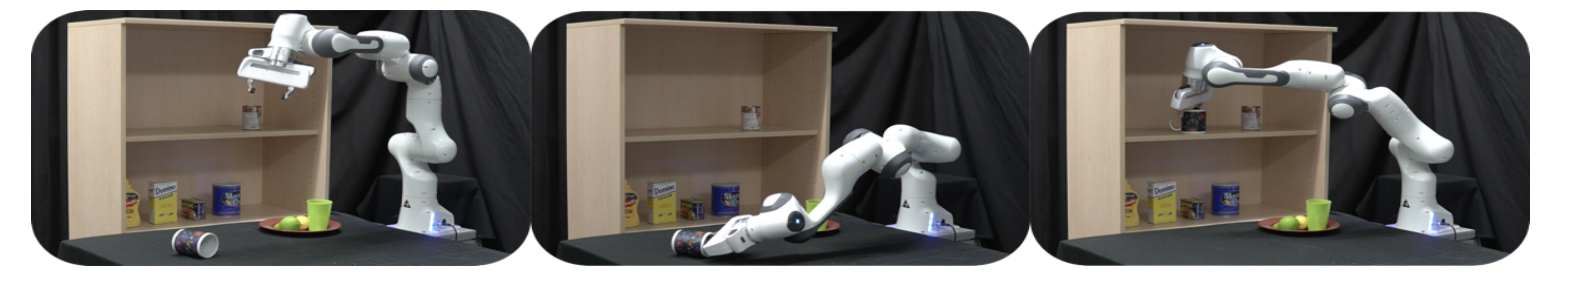
\includegraphics[width=12cm]{pick_place.png}
\end{figure}
\begin{block}{Problem Statement}
How to solve the multi-objective optimization problem of pick and place, where a robot arm can pick up an object and place it somewhere else.
\end{block}
\end{frame}


\begin{frame}{Why is this hard?}
\begin{itemize}
\item The robot must find a grasp pose for the object it must pick up.
\item  The robot must generate a path in order to pick up the object, by taking into consideration its joint and velocity limits and the robot kinematics to accomplish a smooth trajectory(motion optimization).
\item The robot must consider collision avoidance during trajectory generation(often approximated by learning based approaches).
\end{itemize}
\end{frame}


\begin{frame}{Why is this hard?(cont.)}
\begin{itemize} 
\item Most solutions decouple the trajectory generation from the grasp pose estimation(For example what we did with swindepose).
\item This can be problematic because of the disconnected systems. You may infer a grasp pose(there are many possible grasp poses) that has no possible trajectory generation solution in your second system.
\end{itemize}
\end{frame}


\begin{frame}\frametitle{Introduction(cont.)} 
\begin{block}{Solution proposed in paper}
Learning a SE(3) diffusion model for 6DOF grasping, giving rise to a novel framework for joint grasp and motion optimization without needing to decouple grasp selection from trajectory generation. 
\end{block}
\end{frame}    


\begin{frame}{How is this done?}
\begin{itemize}
\item Modify the trajectory generation function(which is a sum of cost functions), by adding another term for the grasp pose selection in cost function form.
\item Use a diffusion model to model the cost function for grasp pose selection.
\item solve for the gradient in the Lie algebra space because very hard otherwise.
\end{itemize}
\end{frame}


\section{Technical Information}
\begin{frame}{Technical Information}
\begin{itemize}
\item LIE Algebra
\item Diffusion
\item Motion Optimization
\end{itemize}  
\end{frame}


\begin{frame}{Inventor of LIE Algebra}
\begin{figure}
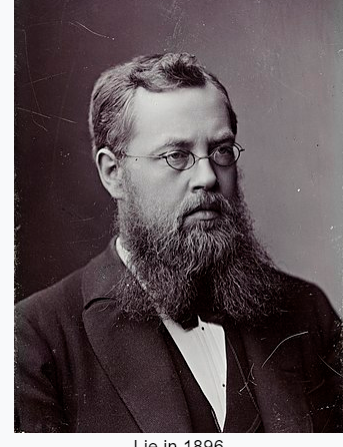
\includegraphics[width=3cm]{lie.png}
\end{figure}
\begin{itemize}
    \item Marius Sophus Lie (17 December 1842 – 18 February 1899) was a Norwegian mathematician. He largely created the theory of continuous symmetry and applied it to the study of geometry and differential equations. He also made substantial contributions to the development of algebra.
\end{itemize}
\end{frame}

\begin{frame}{LIE Algebra Introduction}
\begin{itemize}
\item A lie algebra is a lie group at the identity element.
\item A lie group is a group thats also a smooth(differentiable) manifold(locally similar to a euclidean space).
\item A group is a set with an operation that satisfies the following constraints: the operation is associative and has an identity element, and every element of the set has an inverse element.
\item A lie algebra has an operation called the lie bracket that satisfies the jacobi identity. 
\end{itemize}
\end{frame}


\begin{frame}{LIE Algebra Introduction(cont.)}
\begin{itemize}
    \item $SE(3)$ stands for the special euclidean group in 3 dimension is defined as the set of points that satisfy a point \textbf{H}=$\begin{bmatrix}
        R & t\\
        0 & 1
    \end{bmatrix} \in SE(3)$ where $R \in SO(3)$ and $t \in \mathbb{R}^3$.
    \item $SO(3)$ Stands for the special orthogonal group, and represents the set of orthogonal matrices that have determinant 1(these are all rotation matrices). 
\end{itemize}
\end{frame}


\begin{frame}{LIE Algebra}
\begin{itemize}
    \item The Lie Algebra is the tangent manifold space to the identity element $I= \begin{bmatrix}
        1 & 0 & 0 & 0\\
        0 & 1 & 0 & 0\\
        0 & 0 & 1 & 0\\
        0 & 0 & 0 & 1\\
    \end{bmatrix}$ and is isomorphic to $\mathbb{R}^6$ in which we can apply linear algebra(equations are applied in $\mathbb{R}^6$).
\end{itemize}
\end{frame}


\begin{frame}{LIE Algebra (cont.)}
\begin{block}{A Gaussian distribution on LIE groups}
$q(H|H_{\mu,} \Sigma) \propto exp(-0.5 ||Logmap(H^{-1}_{\mu} H)||^2_{\Sigma^{-1}})$
\end{block}
\begin{itemize}
    \item Logmap : $SE(3) \rightarrow \mathfrak{se}(3)(\text{lie algebra}) \rightarrow \mathbb{R}^6$
    \item $H_\mu \in SE(3)$ is the mean.
    \item $\Sigma \in \mathbb{R}^{6 \times 6}$ is the covariance matrix.
\end{itemize}
\end{frame}


\begin{frame}{Diffusion}
\begin{figure}
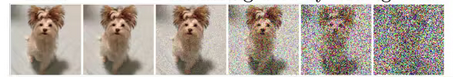
\includegraphics[width=0.8\linewidth]{diffusion_forward.png}
\end{figure}
\begin{itemize}
\item In physics diffusion is the movement of particles move from an area of high concentration to an area of low concentration until equilibrium is reached.
\item Perturb the data distribution with $\rho_D(x)$ with Gaussian noise on L noise scales $\mathcal{N}(0, \sigma^2_kI)$ with $\sigma_1 < \sigma_1 < ... < \sigma_L$.
\item To obtain the noise perturbed distribution: $q_{\sigma_k}(\hat{x})=\int_x \mathcal{N}(\hat{x}|x,\sigma_kI)\rho_D(x)$ where $\hat{x}=x+\epsilon$, $\epsilon \sim \mathcal{N}(0,\sigma_kI)$
\end{itemize}
\end{frame}



\begin{frame}{Denoising Score Matching}
\begin{itemize}
\item estimate the score function(gradient of the log-likelihood) by training the vector field $s_\theta(x,k)$: $s_\theta(x,k) \approx \nabla_x log q_{\sigma_k}(x)$ for all k=1,...,L 
\item Thus, the training objective of DSM is: 
\[ \mathcal{L}_{dsm}=\frac{1}{L} \sum_{k=0}^{L} \mathbb{E}_{x,\hat{x}}[|| s_\theta(x,k) - \nabla_{\hat{x}} log\mathcal{N}(\hat{x}| x, \sigma^2_kI)||] \]
\item $x \sim \rho_D(x)$ and $\hat{x} \sim \mathcal{N}(x, \sigma_k I)$
\end{itemize}
\end{frame}


\begin{frame}{Annealed Langevin Markov Chain Monte Carlo}
\begin{figure}
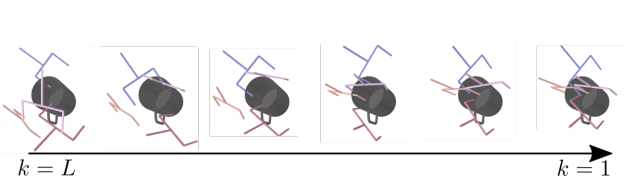
\includegraphics[width=0.8\linewidth]{grasp_diffusion.png}
\end{figure}
\begin{itemize}
    \item Draw sample from the distribution $x_L \sim p_L(x)$ and then simulate the inverse langevian diffusion process for $L$ steps, from $k=L$ to $k=1$
    \item $x_{k-1}=x_k+\frac{\alpha^2_k}{2} s_\theta(x_k, k) + \alpha \epsilon, \epsilon \sim \mathcal{N}(0,I)$
\end{itemize}
\end{frame}


\begin{frame}{From Euclidean Diffusion to SE(3) Diffusion}
\begin{itemize}
    \item A diffusion model in SE(3) is a vector field that outputs a vector $v \in \mathbb{R}^6$, for an arbitrary query point $H \in SE(3)$.
    \item $v=s_\theta (H,k)$ with scalar conditioning variable k determining the current noise scale.
\end{itemize} 
\end{frame}


\begin{frame}{DSM in SE(3) Step 1}
\begin{itemize}
    \item Generate a perturbed data point in SE(3) from the distribution $\hat{H}=q(\hat{H}|H, \sigma_k I)$
    \item Where $\hat{H}=H*Expmap(\epsilon), \epsilon \sim \mathcal{N}(0,\sigma^2_kI)$
    \item Expmap: $\mathbb{R}^6 \rightarrow SE(3)$
\end{itemize} 
\end{frame}


\begin{frame}{DSM in SE(3) Step 2}
\begin{itemize}
    \item Train: \[ \mathcal{L}_{dsm}=\frac{1}{L} \sum^L_{k=0}[|| s_\theta (\hat{H},k)-\frac{Dlogq(\hat{H}|H,\sigma_k I)}{DH} ||] \]
    \item Sampling: \[ H_{k-1}=Expmap(\frac{\alpha^2_k}{2}s_\theta(H,k)+\alpha_k\epsilon)H_k\]
\end{itemize} 
\end{frame}


\begin{frame}\frametitle{Architecture}
\begin{figure}
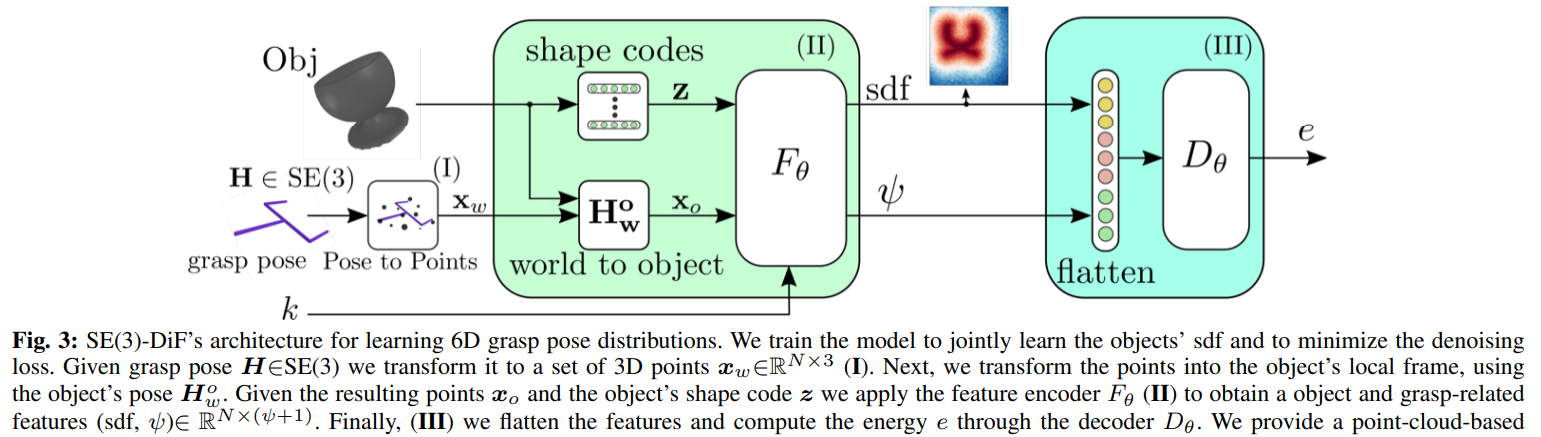
\includegraphics[width=1\linewidth]{architecture.png}
\end{figure}
\begin{itemize}
    \item shape codes are the known shapes of the object in training data
    \item sign distance field(sdf) - A function that takes a position as input and outputs the distance from from that position to the nearest part of the shape(supervised learning pipeline). 
\end{itemize}
\end{frame}


\begin{frame}{Grasp and motion optimization with diffusion models}
\begin{itemize}
\item Given a trajectory $\{q_t\}^T_t=1$ consisting of T way points
\item Using Energy based models (EBM), we model our score function $s_\theta(H,k)=\frac{-DE_\theta (H,k)}{DH}=c_n$ to add it to the motion optimization function.
\item Aim to minimize trajectory: \[ \tau^* = arg min_\tau \sum_j w_j c_j (\tau)\]
\item Finally, we can sample trajectories: \[\tau_{k-1}=\tau_k+\frac{\alpha^2_k}{2} \nabla_{\tau_k}log q(\tau|k ) + \alpha \epsilon, \epsilon \sim \mathcal{N}(0,I)\]
\end{itemize}
\end{frame}


\begin{frame}\frametitle{Training}
\begin{itemize}
    \item Training for  SE(3)-DiF as a 6DoF grasp
pose generative model using the Acronym dataset. This simulation-based dataset contains successful 6DoF grasp
poses for a variety of objects from ShapeNet. It
focuses on the collection of successful grasp poses for 90
different mugs (approximately 90K 6DoF grasp poses).
\end{itemize}
\end{frame}


\begin{frame}\frametitle{Tests}
\begin{enumerate}
\item Generate a set of grasp poses from the
learned models and evaluate on successful grasping and diversity. 
\item Evaluate the quality of the trained model
when used as an additional cost term for grasp and motion
optimization. Compare the performance of
solving a grasp and motion optimization problem jointly
, w.r.t. the state-of-the-art approaches that decouple the grasp selection and motion planning, or heuristically combine them.
\item Validate the performance of the method in a set of real robot experiments.
\end{enumerate}
\end{frame}


\begin{frame}\frametitle{Test 1 (Evaluation of 6DoF grasp pose generation)}
\begin{figure}
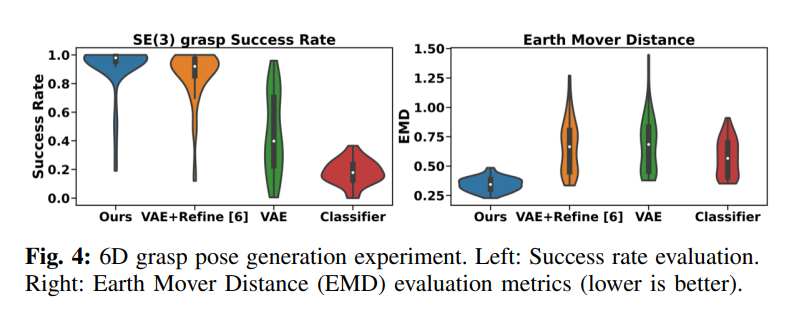
\includegraphics[width=.8\linewidth]{results.png}
\end{figure}
\begin{itemize}
    \item Consider 90 different mugs and evaluate 200
    generated grasps per mug.
    \item The Earth Mover Distance(EMD) measures the divergence
between two empirical probability distributions.
\end{itemize}
\end{frame}


\begin{frame}{Test 2 (Performance on grasp and motion optimization)}
\begin{figure}
    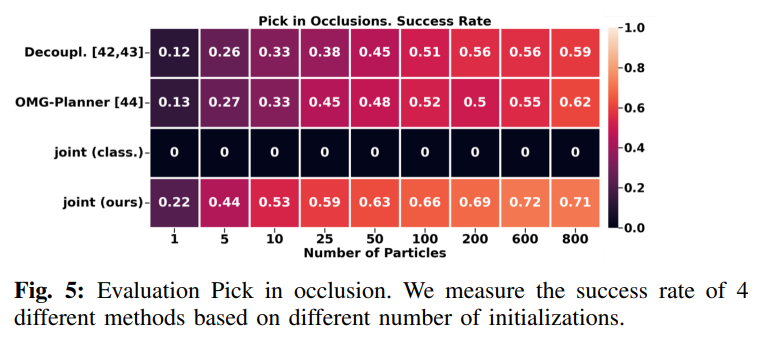
\includegraphics[width=8cm]{results_grasp_with_motion.png}
\end{figure}
    \begin{itemize}
        \item The success is measured based on the robot being
            able to grasp the object at the end of the execution
    \item Generate the trajectories by integrating our
        learned grasp SE(3)-DiF as an additional cost function to
        the motion optimization objective function
    \end{itemize}
\end{frame}

\begin{frame}{Test 2(cont.)}
    \begin{itemize}
    \item Then, given a
    set of initial trajectory samples, obtained from a Gaussian
    distribution with a block diagonal matrix, we apply
    gradient descent methods, to iteratively improve the
    trajectories on the objective function. 
    \item Requires 25 particles(trajectories) to match the success rate of the de-
    coupled approach with 800 particles
    \end{itemize}
\end{frame}

\begin{frame}{Test 3 ( Grasp and motion optimization on real robots)}
    \begin{itemize}
        \item the robot has to pick
up a mug from various poses in a scene without any clutter,
achieved 100\% (20 successes / 20 trials) pickup-success.
\item upside down mugs with 90\% (18/20) success
\item picking in occludes scenes with 95\% (19/20) success
\item having to pick and place the mug in a desired pose inside the shelf of Fig. 1
with 100\% (20/20) success.
\item did not suffer from sim2real discrepancies.
    \end{itemize}
\end{frame}


\section{Conclusion}
\begin{frame}\frametitle{Conclusion}
\begin{figure}
    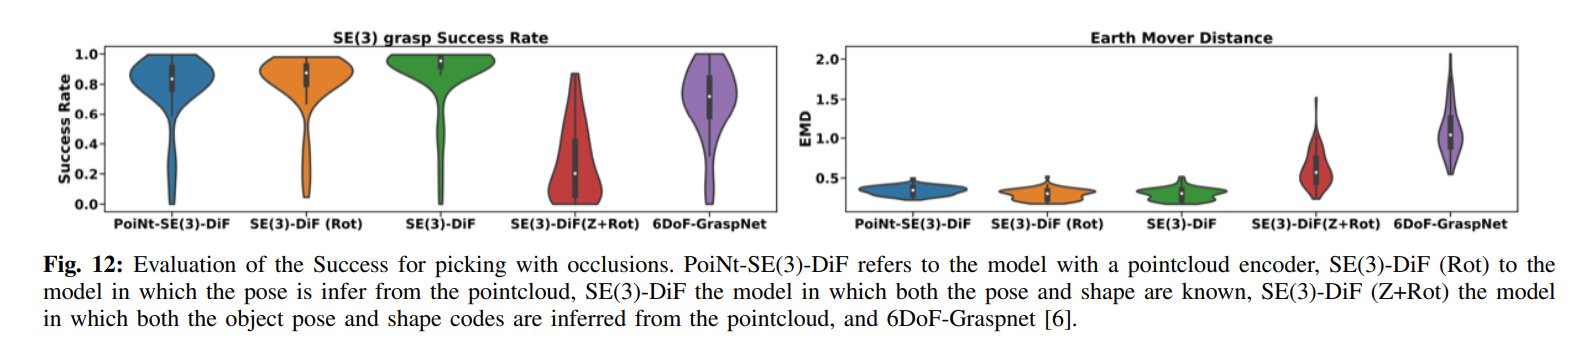
\includegraphics[width=12cm]{results_soa.png}
\end{figure}
\begin{itemize}
\item Comparison to state of the art at the time. 
\end{itemize}
\end{frame}


\begin{frame}
\frametitle{References}
\footnotesize{
\begin{thebibliography}{99} 
\bibitem[Urain, 2023]{p1} Julen Urain, Niklas Funk, Jan Peters, Georgia Chalvatzaki (2023)
\newblock SE(3)-DiffusionFields: Learning smooth cost functions for joint grasp and motion optimization through diffusion
%\newblock \emph{© Springer Science+Business Media, LLC, part of Springer Nature 2020}.
\end{thebibliography}
}
\end{frame}

%https://sites.google.com/view/se3dif


\end{document}
